\chapter{Réalisation}

Ce chapitre décrit l'implémentation \textbf{effective} : organisation du code, choix techniques, points d'implémentation notables et écrans à documenter par captures.

\section{Environnement et choix techniques}

\begin{table}[H]
\centering
\caption{Stack réellement utilisée}
\label{tab:stack}
\begin{tabularx}{\textwidth}{@{}lX@{}}
\toprule
Couche & Choix dans le dépôt \\
\midrule
Frontend & Next.js 16 (App Router), React 19, TypeScript, Tailwind CSS 4, composants d'UI type shadcn / Radix, Lucide, Sonner, \texttt{@react-oauth/google}, socket.io-client \\
Backend & Node.js, Express 5, Mongoose 9, Socket.io 4, JWT, bcryptjs, google-auth-library, \texttt{@google/generative-ai}, Multer, CORS, dotenv \\
Données & MongoDB (URI Atlas en environnement réel) \\
Tests & Jest, Supertest, mongodb-memory-server, Nodemon (dev) \\
Outils hors dépôt & VS Code, Cursor, Antigravity, GitHub, Postman, consoles Google et Atlas \\
\bottomrule
\end{tabularx}
\end{table}

\textbf{Justification succincte.} Next.js fournit le routage et un frontend React moderne, conformément à l'orientation \og React \fg{} du sujet, tout en restant une application web. Express est l'API demandée côté Node. MongoDB Atlas évite d'administrer un serveur local de production. Gemini a été retenu (et utilisé effectivement) plutôt qu'OpenAI. Socket.io couvre le besoin de réactivité du chat et de la file agent. JWT sépare clairement sessions client et sessions agent.

Les alternatives du sujet (Vue.js, Flutter, Firebase, Auth0, Kafka, Docker, Kubernetes, LangChain) \textbf{n'ont pas été mises en œuvre}.

\section{Organisation du code}

Le dépôt est scindé en deux dossiers.

\begin{table}[H]
\centering
\caption{Arborescence simplifiée}
\label{tab:tree}
\begin{tabularx}{\textwidth}{@{}lX@{}}
\toprule
Chemin & Rôle \\
\midrule
\texttt{sinaps-project/app/} & Routes : \texttt{/}, \texttt{/login}, \texttt{/agent}, \texttt{/agent/signup}, \texttt{/admin} \\
\texttt{sinaps-project/components/chat/} & Chat client (fil, en-tête, compositeur, satisfaction, prompts) \\
\texttt{sinaps-project/components/admin/} & Tableau de bord administrateur \\
\texttt{sinaps-project/lib/api.ts} & Client HTTP et gestion des jetons \\
\texttt{sinaps-project/lib/socket.ts} & Client Socket.io \\
\texttt{sinaps-backend/server.js} & HTTP + Socket.io, CORS, montage des routes \\
\texttt{sinaps-backend/models/} & Schémas Mongoose \\
\texttt{sinaps-backend/controllers/} & Logique métier \\
\texttt{sinaps-backend/middleware/auth.js} & Gardes JWT \\
\texttt{sinaps-backend/services/} & \texttt{ragService.js}, \texttt{geminiService.js} \\
\texttt{sinaps-backend/data/knowledgeBase.js} & FAQ d'exemple \\
\texttt{sinaps-backend/tests/} & Suites Jest \\
\texttt{sinaps-backend/seed.js} & Jeu de démonstration \\
\bottomrule
\end{tabularx}
\end{table}

Le frontend écoute par défaut \texttt{NEXT\_PUBLIC\_API\_URL=http://localhost:5000/api}. Le backend écoute le port \textbf{5000}. Un endpoint \texttt{GET /api/health} permet de vérifier que l'API est joignable. Le dépôt fournit aussi des Dockerfiles et un fichier Compose pour le développement, mais aucune configuration de déploiement public n'est présente.

\section{Backend : API REST, middleware et WebSockets}

\subsection{Routes}

\begin{table}[H]
\centering
\caption{Principales routes HTTP}
\label{tab:api}
\small
\begin{tabularx}{\textwidth}{@{}llX@{}}
\toprule
Méthode & Chemin & Rôle \\
\midrule
GET & \texttt{/api/health} & Santé du serveur \\
POST & \texttt{/api/users/find-or-create} & Session client (Google ou e-mail) \\
POST & \texttt{/api/conversations/find-or-create} & Conversation active du client \\
GET & \texttt{/api/conversations} & Liste (agent/admin), filtre \texttt{status}, \texttt{search} \\
GET & \texttt{/api/conversations/:id} & Fil + messages (propriétaire ou staff) \\
PATCH & \texttt{/api/conversations/:id/escalate} & Vers humain \\
PATCH & \texttt{/api/conversations/:id/de-escalate} & Retour IA \\
PATCH & \texttt{/api/conversations/:id/assign} & Assignation d'agent \\
PATCH & \texttt{/api/conversations/:id/close} & Clôture $\pm$ satisfaction \\
POST & \texttt{/api/messages} & Envoi ; déclenche l'IA si besoin \\
POST & \texttt{/api/upload} & Fichier (session requise) \\
POST & \texttt{/api/agents/signup} & Inscription \texttt{pending} \\
POST & \texttt{/api/agents/login} & JWT staff \\
GET & \texttt{/api/agents} & Liste (admin) \\
PATCH & \texttt{/api/agents/:id/approve} & Validation \\
DELETE & \texttt{/api/agents/:id} & Rejet (suppression) \\
GET & \texttt{/api/stats} & Indicateurs admin \\
\bottomrule
\end{tabularx}
\end{table}

\subsection{Temps réel}

Lors d'une connexion Socket.io, le client peut \texttt{join\_conversation} / \texttt{leave\_conversation}. Le backend émet \texttt{message\_received} et \texttt{conversation\_updated} vers la salle, et \texttt{conversation\_created} / \texttt{conversation\_updated} en global pour les listes.

\subsection{Statistiques}

\texttt{getStats} calcule : nombre total de conversations, résolues par IA, résolues par un humain, moyenne des notes renseignées, et un \textbf{temps de réponse moyen} (écart entre le premier message client et la première réponse IA ou humaine), en une passe sur les messages plutôt qu'en boucle na\"ive requête par conversation.

\subsection{Téléversement}

Multer enregistre les fichiers avec un nom unique. Types acceptés : images, vidéos, PDF, Word. Taille maximale configurable (\texttt{MAX\_UPLOAD\_SIZE\_MB}, défaut 15~Mo). Le filtrage repose sur le type MIME déclaré par le client : il écarte les usages accidentels, sans constituer une analyse d'octets magiques.

\section{Moteur IA}

Le fichier \texttt{geminiService.js} enchaîne : retrieval $\rightarrow$ construction du prompt $\rightarrow$ essai de modèles Gemini $\rightarrow$ repli RAG textuel. La FAQ d'exemple couvre notamment : suivi de commande, retard, remboursement, mot de passe, code promo. Elle n'est pas un corpus métier confidentiel de SINAPS TEC.

\section{Frontend}

\subsection{Espace client}

Après identification (\texttt{ClientEntryForm}, bouton Google et/ou formulaire), \texttt{SupportChatApp} charge le fil, affiche \texttt{ChatThread}, \texttt{QuickPrompts}, \texttt{MessageComposer}, et les actions d'escalade / désescalade dans \texttt{ChatHeader}. Un dialogue de satisfaction s'ouvre à la clôture.

\begin{figure}[H]
  \centering
  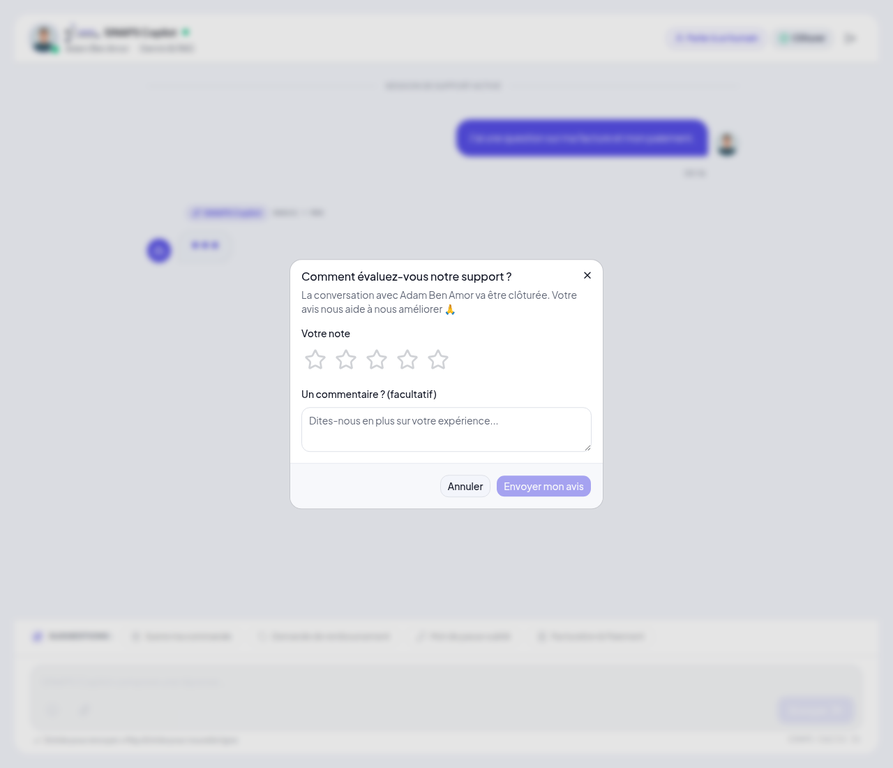
\includegraphics[width=0.9\textwidth]{images/sinaps-satisfaction-dialog.png}
  \caption{Évaluation de la satisfaction à la clôture d'une conversation}
  \label{fig:satisfaction-dialog}
\end{figure}

Les réponses IA peuvent porter des \textbf{actions rapides} : confirmer que la réponse a suffi, poser une autre question ou demander un agent humain. Une action est envoyée comme message client et son état de chargement est affiché ; les boutons ne sont proposés que sur le dernier message IA éligible. Le compositeur est verrouillé pendant la génération IA afin d'éviter les doublons.

\begin{figure}[H]
  \centering
  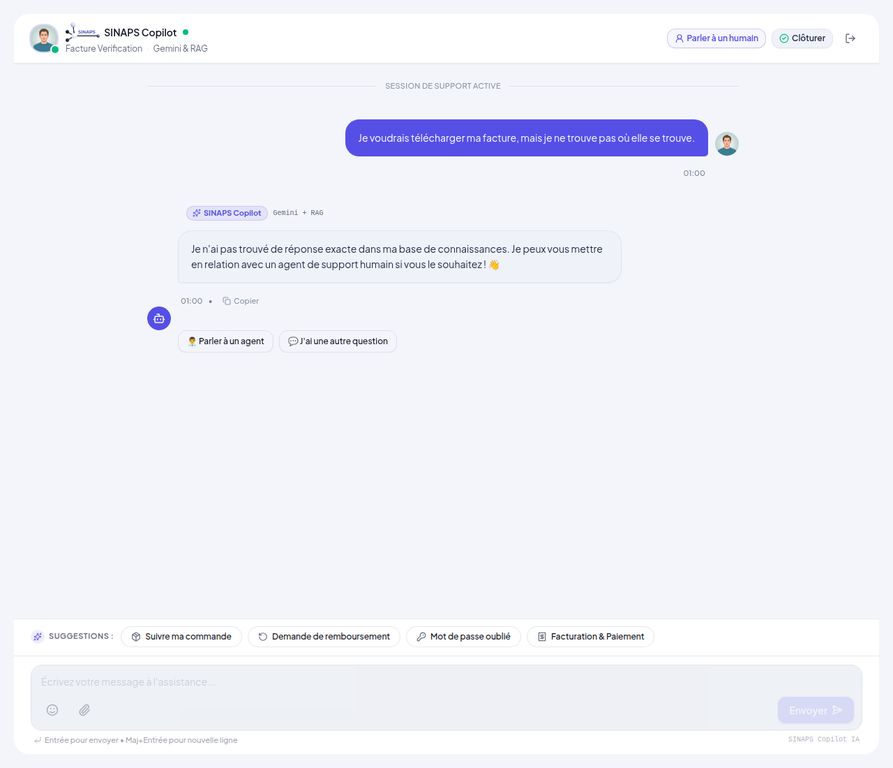
\includegraphics[width=0.9\textwidth]{images/sinaps-client-chat-ai.png}
  \caption{Conversation client avec réponse RAG/Gemini et actions rapides}
  \label{fig:client-chat-ai}
\end{figure}

\subsection{Espace agent}

La page \texttt{/agent} est protégée (\texttt{AuthGuard}). L'agent se connecte sur \texttt{/login}. L'inscription se fait sur \texttt{/agent/signup} (compétences en texte). Tant que le compte est \texttt{pending}, le login renvoie une erreur 403.

\begin{figure}[H]
  \centering
  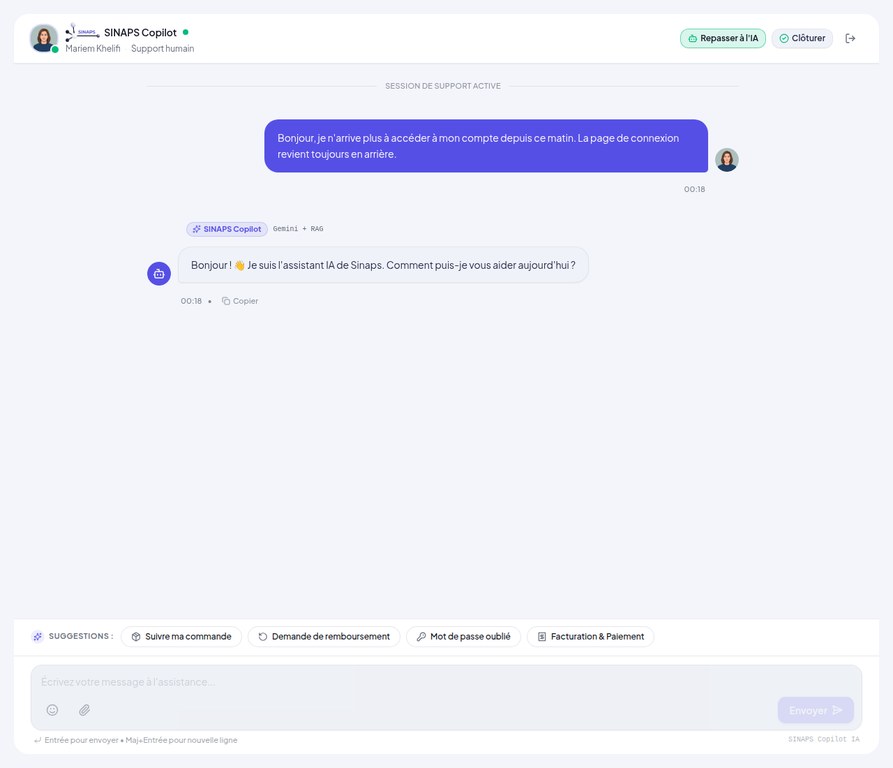
\includegraphics[width=0.9\textwidth]{images/sinaps-human-escalation.png}
  \caption{Escalade d'une conversation vers la file des agents}
  \label{fig:human-escalation}
\end{figure}

\subsection{Espace administrateur}

Le tableau de bord affiche les indicateurs SLA calculés, la liste des agents à valider (compétences en badges), et un historique avec recherche (nom / e-mail client) et onglets de statut. Les conversations marquées comme données de test sont exclues des indicateurs et des listes opérationnelles par défaut. Les dernières corrections ont également stabilisé le chargement concurrent des conversations, le rendu des horodatages et les avatars de repli côté client.

\begin{figure}[H]
  \centering
  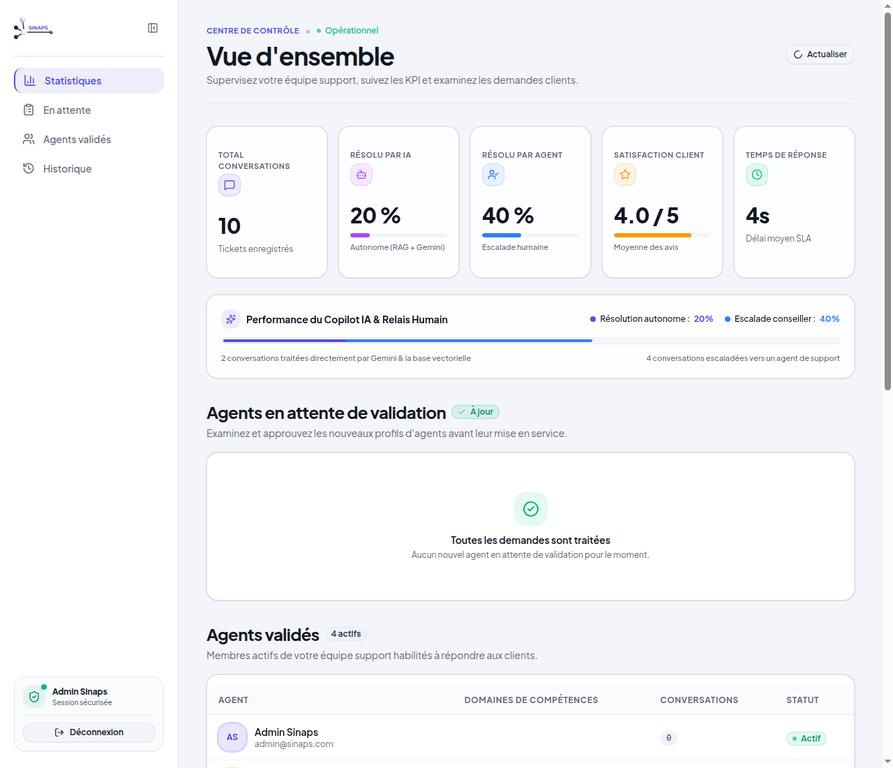
\includegraphics[width=0.95\textwidth]{images/sinaps-admin-dashboard.png}
  \caption{Tableau de bord administrateur de SINAPS TEC}
  \label{fig:admin-dashboard}
\end{figure}

\section{Données de démonstration}

Le script \texttt{npm run seed} recrée des comptes d'exemple (mot de passe de seed : \texttt{password123}) : administrateur \texttt{admin@sinaps.com}, agents validés et un agent en attente, plus des utilisateurs et conversations de démonstration. Ces comptes servent aux captures et aux tests manuels ; ils ne constituent pas une population réelle de production.

\section{Captures d'écran à insérer}

Les captures ci-dessous sont des \textbf{recommandations de documentation}, et non des résultats inventés. Les captures importantes montrent les parcours fonctionnels principaux ; les captures optionnelles peuvent être regroupées ou remplacées par les diagrammes déjà présents au chapitre~3.

\begin{enumerate}[leftmargin=1.6em]
  \item \textbf{Important --- Chat IA et actions rapides}. Capture de \texttt{/} après une question documentée, avec réponse IA, horodatage et boutons « C'est ce qu'il me fallait », « autre question » et « agent ». Placement : après le paragraphe sur l'espace client. Caption : \textit{Conversation client avec réponse RAG/Gemini et actions rapides}. Label : \texttt{fig:client-chat-ai}.
  \item \textbf{Important --- Escalade et espace agent}. Capture de \texttt{/} puis \texttt{/agent} montrant le statut en attente, la file et une réponse humaine. Placement : après le paragraphe sur l'espace agent. Caption : \textit{Escalade d'une conversation vers la file des agents}. Label : \texttt{fig:human-escalation}.
  \item \textbf{Important --- Dashboard administrateur}. Capture de \texttt{/admin} montrant les KPI, la validation des agents et l'historique filtrable. Placement : après le paragraphe sur l'espace administrateur. Caption : \textit{Tableau de bord administrateur de SINAPS TEC}. Label : \texttt{fig:admin-dashboard}.
  \item \textbf{Important --- Clôture et satisfaction}. Capture du dialogue de notation 1--5 avec commentaire facultatif. Placement : après le paragraphe sur la satisfaction. Caption : \textit{Évaluation de la satisfaction à la clôture d'une conversation}. Label : \texttt{fig:satisfaction-dialog}.
  \item \textbf{Optionnel --- Identification client}. Capture de \texttt{/} avant connexion, avec Google Sign-In et formulaire direct. Placement : au début de la sous-section « Espace client ». Caption : \textit{Identification du client par Google ou formulaire}. Label : \texttt{fig:client-auth}.
  \item \textbf{Optionnel --- Pièce jointe et profils}. Capture du fil avec une pièce jointe et les avatars client/agent. Placement : après le paragraphe sur l'espace client. Caption : \textit{Message avec pièce jointe et avatars persistés}. Label : \texttt{fig:message-attachment-avatar}.
  \item \textbf{Optionnel --- Inscription et validation}. Capture de \texttt{/agent/signup} puis de la table des agents en attente. Placement : après le paragraphe sur l'espace administrateur. Caption : \textit{Inscription d'un agent et validation administrative}. Label : \texttt{fig:agent-approval}.
\end{enumerate}

Un \textbf{diagramme de séquence} reste préférable à une capture pour expliquer le flux interne RAG $\rightarrow$ Gemini $\rightarrow$ persistance $\rightarrow$ Socket.io ; la figure~\ref{fig:seq-ia} remplit déjà ce rôle.

\section{Mise en route (développement local)}

\begin{lstlisting}[caption={Démarrage local (d'après le README du projet)},label=lst:run]
# MongoDB Atlas : renseigner MONGO_URI
cd sinaps-backend && npm install && npm run seed && npm run dev
cd sinaps-project && npm install && npm run dev
\end{lstlisting}

Variables nécessaires côté backend : \texttt{PORT}, \texttt{MONGO\_URI}, \texttt{JWT\_SECRET}, \texttt{GEMINI\_API\_KEY}, \texttt{GOOGLE\_CLIENT\_ID} ; côté frontend : \texttt{NEXT\_PUBLIC\_API\_URL}, \texttt{NEXT\_PUBLIC\_GOOGLE\_CLIENT\_ID}. Sans clés Google/Gemini, des modes dégradés existent (identification directe, réponses RAG locales). Le dépôt confirme l'intégration de Google Sign-In, Gemini et MongoDB Atlas, mais ne fournit pas de compte rendu détaillé d'une recette manuelle en conditions réelles.
